%%% Local Variables:
%%% mode: latex
%%% TeX-master: t
%%% End:

\documentclass[master,xetex]{thuthesis}
% \documentclass[%
%   bachelor|master|doctor|postdoctor, % mandatory option
%   xetex|pdftex|dvips|dvipdfm, % optional
%   secret,
%   openany|openright,
%   arialtoc,arialtitle]{thuthesis}

% 所有其它可能用到的包都统一放到这里了,可以根据自己的实际添加或者删除。
\usepackage[
addfootnotetoref
]{thutils}

\usepackage[xetex,hyperref]{xcolor}
\usepackage{tikz}

\newcommand{\TODO}{ \textcolor{blue}{TODO} }
\colorlet{BLUE}{blue}

%--------------------------------------------------------------------------
% 自定义函数

%bracket系列
\newcommand{\bracket}[4]
{\ensuremath{%
\ifthenelse{\equal{#1}{n}}{#3 #2 #4}{}%
\ifthenelse{\equal{#1}{b}}{\bigl#3 #2 \bigr#4}{}%
\ifthenelse{\equal{#1}{B}}{\Bigl#3 #2 \Bigr#4}{}%
\ifthenelse{\equal{#1}{bg}}{\biggl#3 #2 \biggr#4}{}%
\ifthenelse{\equal{#1}{Bg}}{\Biggl#3 #2 \Biggr#4}{}%
}}

\newcommand{\pbracket}[2]{\bracket{#1}{#2}{(}{)}}
\newcommand{\Sbracket}[2]{\bracket{#1}{#2}{[}{]}}
\newcommand{\Bbracket}[2]{\bracket{#1}{#2}{\lbrace}{\rbrace}}
\newcommand{\vbracket}[2]{\bracket{#1}{#2}{|}{|}}

\newcommand{\getsize}[2]
{%
\ifthenelse{\equal{#1}{n}}{#2}{}%
\ifthenelse{\equal{#1}{b}}{\big#2}{}%
\ifthenelse{\equal{#1}{B}}{\Big#2}{}%
\ifthenelse{\equal{#1}{bg}}{\bigg#2}{}%
\ifthenelse{\equal{#1}{Bg}}{\Bigg#2}{}%
}

\newcommand{\pb}[2][n]{\pbracket{#1}{#2}}
\newcommand{\Sb}[2][n]{\Sbracket{#1}{#2}}
\newcommand{\Bb}[2][n]{\Bbracket{#1}{#2}}
\newcommand{\vb}[2][n]{\vbracket{#1}{#2}}

\newcommand{\diff}[1]{\mathrm{d}#1}

\usepackage{datetime}
\newdateformat{mydate}{\THEYEAR-\twodigit{\THEMONTH}-\twodigit{\THEDAY}}
\newtimeformat{mytime}{\twodigit{\THEHOUR}:\twodigit{\THEMINUTE}}
\settimeformat{mytime}

\usepackage[draft=true,allpages=true]{draftmark}
\draftmarksetup{angle=45,grayness=0.9,
mark={DRAFT \\ \huge 编译时间:\mydate\today\hspace{5pt} \currenttime}}

%只显示三层目录
\setcounter{tocdepth}{2}

\begin{document}

% 定义所有的eps文件在 figures 子目录下
\graphicspath{{figures/}}


%%% 封面部分
\frontmatter

%%% Local Variables:
%%% mode: latex
%%% TeX-master: t
%%% End:
\secretlevel{绝密} \secretyear{2100}

\ctitle{清华大学学位论文 \LaTeX\ 模板\\使用示例文档}
% 根据自己的情况选,不用这样复杂
\makeatletter
\ifthu@bachelor\relax\else
  \ifthu@doctor
    \cdegree{工学博士}
  \else
    \ifthu@master
      \cdegree{工学硕士}
    \fi
  \fi
\fi
\makeatother


\cdepartment[计算机]{计算机科学与技术系}
\cmajor{计算机科学与技术}
\cauthor{薛瑞尼} 
\csupervisor{郑纬民教授}
% 如果没有副指导老师或者联合指导老师,把下面两行相应的删除即可。
\cassosupervisor{陈文光教授}
\ccosupervisor{某某某教授}
% 日期自动生成,如果你要自己写就改这个cdate
%\cdate{\CJKdigits{\the\year}年\CJKnumber{\the\month}月}

% 博士后部分
% \cfirstdiscipline{计算机科学与技术}
% \cseconddiscipline{系统结构}
% \postdoctordate{2009年7月——2011年7月}

\etitle{An Introduction to \LaTeX{} Thesis Template of Tsinghua University} 
% 这块比较复杂,需要分情况讨论:
% 1. 学术型硕士
%    \edegree:必须为Master of Arts或Master of Science(注意大小写)
%              “哲学、文学、历史学、法学、教育学、艺术学门类,公共管理学科
%               填写Master of Arts,其它填写Master of Science”
%    \emajor:“获得一级学科授权的学科填写一级学科名称,其它填写二级学科名称”
% 2. 专业型硕士
%    \edegree:“填写专业学位英文名称全称”
%    \emajor:“工程硕士填写工程领域,其它专业学位不填写此项”
% 3. 学术型博士
%    \edegree:Doctor of Philosophy(注意大小写)
%    \emajor:“获得一级学科授权的学科填写一级学科名称,其它填写二级学科名称”
% 4. 专业型博士
%    \edegree:“填写专业学位英文名称全称”
%    \emajor:不填写此项
\edegree{Doctor of Engineering} 
\emajor{Computer Science and Technology} 
\eauthor{Xue Ruini} 
\esupervisor{Professor Zheng Weimin} 
\eassosupervisor{Chen Wenguang} 
% 这个日期也会自动生成,你要改么?
% \edate{December, 2005}

% 定义中英文摘要和关键字
\begin{cabstract}
  论文的摘要是对论文研究内容和成果的高度概括。摘要应对论文所研究的问题及其研究目
  的进行描述,对研究方法和过程进行简单介绍,对研究成果和所得结论进行概括。摘要应
  具有独立性和自明性,其内容应包含与论文全文同等量的主要信息。使读者即使不阅读全
  文,通过摘要就能了解论文的总体内容和主要成果。

  论文摘要的书写应力求精确、简明。切忌写成对论文书写内容进行提要的形式,尤其要避
  免“第 1 章……;第 2 章……;……”这种或类似的陈述方式。

  本文介绍清华大学论文模板 \thuthesis{} 的使用方法。本模板符合学校的本科、硕士、
  博士论文格式要求。

  本文的创新点主要有:
  \begin{itemize}
    \item 用例子来解释模板的使用方法;
    \item 用废话来填充无关紧要的部分;
    \item 一边学习摸索一边编写新代码。
  \end{itemize}

  关键词是为了文献标引工作、用以表示全文主要内容信息的单词或术语。关键词不超过 5
  个,每个关键词中间用分号分隔。(模板作者注:关键词分隔符不用考虑,模板会自动处
  理。英文关键词同理。)
\end{cabstract}

\ckeywords{\TeX, \LaTeX, CJK, 模板, 论文}

\begin{eabstract} 
   An abstract of a dissertation is a summary and extraction of research work
   and contributions. Included in an abstract should be description of research
   topic and research objective, brief introduction to methodology and research
   process, and summarization of conclusion and contributions of the
   research. An abstract should be characterized by independence and clarity and
   carry identical information with the dissertation. It should be such that the
   general idea and major contributions of the dissertation are conveyed without
   reading the dissertation. 

   An abstract should be concise and to the point. It is a misunderstanding to
   make an abstract an outline of the dissertation and words ``the first
   chapter'', ``the second chapter'' and the like should be avoided in the
   abstract.

   Key words are terms used in a dissertation for indexing, reflecting core
   information of the dissertation. An abstract may contain a maximum of 5 key
   words, with semi-colons used in between to separate one another.
\end{eabstract}

\ekeywords{\TeX, \LaTeX, CJK, template, thesis}

%\makecover

% 目录
\tableofcontents

% 符号对照表
%\begin{denotation}

\item[HDF] Hierarchical Data Format
\item[GPU] Graphics Processing Unit
\item[CPU] Central processing unit
\item[CG] Conjugate Gradient
\item[\ProgramName] \ProgramFullName

\item[PWR] Pressurized Water Reactor
\item[API] Application Programming Interface
\item[CUDA] Compute Unified Device Architecture
\item[MPI] Message Passing Interface
\item[SIMD] Single instruction, multiple data
\item[MIMD] multiple instruction, multiple data
\item[ADI] Alternating direction implicit method
\item[SM] Streaming Multiprocessor
\item[SMX] Next Generation Streaming Multiprocessor
\item[PTX] Parallel Thread Execution
\item[ISA] Instruction Set Architecture
\item[JIT] Just-in-time Compiler
\item[GMRES] Generalized Minimal RESidual method

\end{denotation}



%%% 正文部分
\mainmatter

\chapter{引言}
\section{研究背景}
\section{国内外研究现状}
\section{研究内容和论文组织结构}




\chapter{GPU科学计算简介}

\section{CUDA简介}

\subsection{CUDA总体设计}

CUDA翻译为统一计算设备架构,本身定位做一种包含CPU和GPU的编程模型,
不过实际上一般只用作GPU编程和GPU、CPU通讯编程。

CUDA把设备资源分为主机端和GPU端两部分,
主机端包含CPU、内存等正常C/C++程序可以访问到的资源,
GPU端包含多个SM(Streaming Multiprocessor)
或SMX(Next Generation Streaming Multiprocessor)
\footnote{从 NVIDIA显卡的 Kepler 架构开始,SM的规格大幅改变,改称为SMX。
为方便起见以下不再提SM,提到SMX时也包含SM。}
、显存等资源。

其中SMX代表GPU核心内的一个相对独立的向量处理单元,
类似传统的向量机中央处理器,这些SMX位于GPU的核心芯片内。
显存位于显卡PCB上,并被所有的SMX共享。

显存和主机内存是独立的,有各自的地址空间,
CPU端的代码不能直接读写显存,
GPU端的代码也不能直接读写内存,
需要程序员手工在显存和内存之间做数据传输。
CUDA允许在主机端申请所谓的\emph{页锁定主机内存}(Page-Locked Host Memory),
并允许GPU端直接访问,
由显卡驱动负责在内存和显卡之间进行自动数据传输。
此外,对于通用计算专用的Tesla显卡,
CUDA可以开启Unified Virtual Address Space功能,
即对内存和显存统一编址访问,可以省去一些编程上的繁琐操作。
\cite{cudadoc-cprogrammingguide}

\subsubsection{Global函数}

GPU上执行的代码需要放在专门的Kernel函数中,
这些函数在CUDA使用\_\_global\_\_进行标识,所以又称global函数。
Global函数只能由CPU端的代码通过特殊方式调用。
在CUDA 5.0之前global函数间不能相互调用,
global函数只能调用一种有\_\_device\_\_标识的函数(以下称为device函数)。
CUDA 5.0引入了Dynamic Parallelism功能,
允许在global函数内调用global函数,并定义了对应的语义,
该功能依赖计算能力\footnote{NVIDIA对其发布的GPU核心的功能进行划分的标准,当前Kepler架构的计算能力为3.0-3.5。}%
为3.5的GPU核心(如GK110,对应的显卡有GTX Titian、Tesla K20等),
详见文献\onlinecite{cudadoc-dynamicparallelism}。

Global函数是GPU上运行的程序的最基本单元,虽然global函数可以调用device函数,
但被调用的device函数的各种运行时配置都是依赖于直接或间接调用它的global函数。

Global函数实际运行时可以被一组线程同步执行,类似传统的向量机,
同步执行的线程数量在调用global函数的时候进行设置。

CUDA将运行一个global函数的线程分Grid、Block两个层级进行组织:
Grid代表所有参与的线程,一个Grid包含一个或多个Block,每个Block在Grid内都有自己的编号,
CUDA提供的Block编号可以是1维、2维或3维整数;
一个Block又包含一个或多个Thread,每个Thread在Block内也有自己的编号,
CUDA提供的Thread编号同样是1维、2维或3维整数,
这里的Thread就是一个实际的硬件线程,有自己的寄存器组等资源。
一个实际的线程组设置见\floatref{fig:gpu.cuda.blocks}。

\begin{figure}
\centering
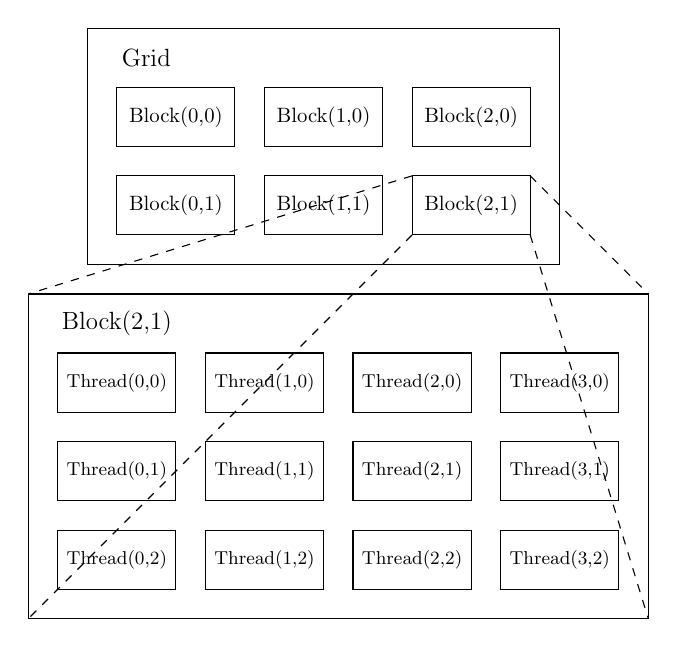
\begin{tikzpicture}[scale=0.75, transform shape]
\def\TextBox#1#2#3{
\draw  (#1,#2) rectangle (#1+2,#2+1);
\node at (#1+1, #2+0.5) {#3};
}

\foreach \x in {0,...,2}
  \foreach \y in {0,...,1}
  {
    \TextBox{\x*2.5+1}{-\y*1.5+3}{Block(\x,\y)}
  }
\draw  (0.5,5) rectangle (8.5,1);
\node at (1.5,4.5) {\large Grid};

\foreach \x in {0,...,3}
  \foreach \y in {0,...,2}
  {
    \TextBox{\x*2.5}{-\y*1.5-1.5}{\small Thread(\x,\y)}
  }
\draw  (-0.5,0.5)  rectangle (10,-5);
\node at (1,0) {\large Block(2,1)};

\draw [dashed]  (6,2.5) edge (-0.5,0.5);
\draw [dashed]  (8,2.5) edge (10,0.5);
\draw [dashed]  (6,1.5) edge (-0.5,-5);
\draw [dashed]  (8,1.5) edge (10,-5);
\end{tikzpicture}
\caption[线程组层次结构示意图]{\label{fig:gpu.cuda.blocks}线程组层次结构示意图
\cite{cudadoc-cprogrammingguide}}
\end{figure}

同一个global函数调用时所涉及的线程均使用global函数的参数作为输入,
CUDA提供threadIdx、blockIdx等变量在代码中区分各个线程。
线程以Block为单元分配给GPU上的各个SMX独立执行,
Block之间没有任何直接的同步方式,
程序员不需要知道也不应该猜测各Block是如何在各个SMX执行的。
需要说明的是:强行使用显存作为Block间的同步可能会导致各SMX死锁。
实际Block间同步的最主要方式就是等待该global函数执行完,
此时所有Block状态都是确定的,即已经执行完。

这样GPU或驱动就可以根据实际GPU核心上的SMX数量来具体配置各Block是如何在SMX上执行的,
使得当SM数量不超过Block数量时global函数有了一定的并行扩展性,
见\floatref{fig:gpu.cuda.scalability}。
由于每个Block是运行在一个实际SMX上的,
所以SMX的寄存器、共享存储空间等资源会对Block的大小(包含的Thread数量)有一定的限制,
而CUDA对Grid大小(包含的Block数量)的限制则很小。
NVIDIA这样做是为了通过强制程序员对计算任务进行分割的方式获得了一定的程序并行扩展性,
同时也简化了同一系列不同规格GPU的设计,即通过增减SMX的数量来控制GPU计算能力。

\begin{figure}
\centering
\begin{tikzpicture}[scale=0.6, transform shape]
\def\TextBox#1#2#3{
\draw  (#1,#2) rectangle (#1+2,#2+1);
\node at (#1+1, #2+0.5) {#3};
}

\foreach \x in {0,...,3}
  \foreach \y in {0,...,1}
  {
    \TextBox{\x*2.5+1}{-\y*1.5+3}{Block(\x,\y)}
  }
\draw  (0.5,5) rectangle (11,1);
\node at (3,4.5) {\large Kernel函数的Grid};

\draw [dashed] (-3,-4) -- (16.5,-4);

\draw  (-1,-3.5) rectangle (4.5,-1);
\node at (1.5,-1.5) {\large 2个SMX的GPU};
\draw [-latex new, arrow head=3mm] (7,1) -- (9.5,-1);
\foreach \x in {0,...,1}
{
  \TextBox{\x*2.5-0.5}{-3}{SMX \x}
}
\foreach \t in {0,...,3}
{
  \foreach \x in {0,...,1}
  {
    \TextBox{\x*2.5-0.5}{-\t*2-6}{Block(\t,\x)}
  }
  \draw  (-1,-\t*2-4.75) rectangle (4.5,-\t*2-6.25);
}

\draw  (5.5,-3.5) rectangle (16,-1);
\node at (8,-1.5) {\large 4个SMX的GPU};
\draw [-latex new, arrow head=3mm] (3.5,1) -- (2,-1);
\foreach \x in {0,...,3}
{
  \TextBox{\x*2.5+6}{-3}{SMX \x}
}
\foreach \t in {0,...,1}
{
  \foreach \x in {0,...,3}
  {
    \TextBox{\x*2.5+6}{-\t*2-6}{Block(\x,\t)}
  }
  \draw  (5.5,-\t*2-4.75) rectangle (16,-\t*2-6.25);
}

\draw [dashed,-latex new, arrow head=3mm] (-1.5,-4.5) -- (-1.5,-13);
\foreach \t in {0,...,3}
{
  \node at  (-2.5,-\t*2-5.5) {\Large t=\t};
}

\draw (5,-0.5) -- (5,-12.5);
\end{tikzpicture}
\caption[CUDA程序的扩展性示意图]{\label{fig:gpu.cuda.scalability}CUDA程序的扩展性示意图
\cite{cudadoc-cprogrammingguide}}
\end{figure}

总的来说,GPU核心相当于一组不能单独编程的、以显存作为共享存储器的、带有自动负载平衡的小型向量机组。


\subsection{CUDA的GPU设备模型}

\begin{figure}
\centering
\begin{tikzpicture}[scale=0.75, transform shape]
%15*SMX
\def\SMX#1#2{
\draw  (#1+0, #2) rectangle (#1+1, #2+1);
\node at (#1+0.5, #2+0.5) {\small SMX};
}
\def\len{1.5}
\foreach \x in {0,...,8}
{ \SMX{\x*\len}{0} }
\foreach \x in {0,...,7}
{ \SMX{\x*\len+0.75}{-3} }

%L2 Cache
\draw  (0,-0.5) rectangle (13,-1.5);
\node at (6.5,-1) {L2缓存};


\def\Memory#1#2{
\draw  (#1,#2) rectangle (#1+2,#2+1);
\node at (#1+1,#2+0.5) {\small 显存控制器};
}
\foreach \i in {0,1,2}
{ \Memory{-2.5}{-\i*1.5} }
\foreach \i in {0,1,2}
{ \Memory{13.5}{-\i*1.5} }

\draw  (-2.5,2) rectangle (15.5,1.5);
\node at (6.5,1.75) {线程调度器(GigaThread Engine)};

\draw  (-2.5,3) rectangle (15.5,2.5);
\node at (6.5,2.75) {PCI Express 3.0接口};

\draw  (-3,4) rectangle (16,-3.5);
\node at (-1.5,3.5) {\Large GK110};
\end{tikzpicture}
\caption[GK110结构示意图]{\label{fig:gpu.cuda.gk110}GK110结构示意图
\cite{cudadoc-KeplerGK110ArchitectureWhitepaper}}
\end{figure}

GPU是由多个SMX组成的,例如Kepler架构GK110核心
(见\floatref{fig:gpu.cuda.gk110})就包含15个SMX,
其中每个SMX(见\floatref{fig:gpu.cuda.smx})
含有192个CUDA Core单元(支持单精度、整数计算,图示中Core)、
64个双精度浮点计算单元(图示中DP Unit)、
32个特殊函数计算单元(图示中SFU)、
32个读取/存储单元(图示中LD/ST),
4个Wrap调度器,65536个32bit寄存器。
SMX以32个Thread为一组(称为wrap)来调度Block中的线程,
每个SMX有4个wrap调度器和8个指令分派单元,这使得SMX可以同时执行4个wrap,
每个周期中每个wrap最多可以有两条不相关的指令被同时分派。
\cite{cudadoc-KeplerGK110ArchitectureWhitepaper}

\begin{figure}
\centering
%\includegraphics[scale=0.6]{smx.png}
\begin{tikzpicture}[scale=0.7, transform shape]
\def\TextBox#1#2#3#4
{
  \draw (#1,#2) rectangle (#1+#3,#2+1);
  \node at (#1+#3/2, #2+0.5) {#4};
}

\def\CoreLine#1#2
{
\foreach \i in {0,...,2}
{ \TextBox{#1+\i*1.5+0}{#2+0}{1}{Core} }
\TextBox{#1+4.5}{#2+0}{2}{DP Unit}

\foreach \i in {0,...,2}
{ \TextBox{#1+\i*1.5+7}{#2+0}{1}{Core} }
\TextBox{#1+11.5}{#2+0}{2}{DP Unit}

\TextBox{#1+14}{#2+0}{1.5}{LD/ST}
\TextBox{#1+16}{#2+0}{1}{SFU}
}

\CoreLine{0}{0}

\CoreLine{0}{-4}

\draw [decorate, decoration={brace, amplitude=10pt}] (-0.5,-4.25) -- (-0.5,1.25);
\node [left]at (-1,-1.5) {\large 32组};
\draw [loosely dashed] (0.5,-0.5) -- (0.5,-2.5);
\draw [loosely dashed] (8,-0.5) -- (8,-2.5);
\draw [loosely dashed] (16.5,-0.5) -- (16.5,-2.5);

\draw  (-0.5,2.5) rectangle (17.5,1.5);
\node at (8,2) {\large 寄存器文件(65536个 32bit寄存器)};

\foreach \x in {0,...,3}
{
  \def\xlen{4.5}
  \draw  (\x*\xlen-0.25,4) rectangle (\x*\xlen-0.25+4,3);
  \node  at (\x*\xlen+1.75,3.5) {\large Wrap调度器}; 
}
\draw  (-0.5,4.5) rectangle (17.5,5.5);
\node at (8,5) {\large 指令缓存};

\draw  (17.5,-4.5) rectangle (-0.5,-5.5);
\draw  (17.5,-6) rectangle (-0.5,-7);
\draw  (17.5,-7.5) rectangle (-0.5,-8.5);
\node at (8,-5) {\large 内部互联网络};
\node at (8,-6.5) {\large 64KB 共享存储区 / L1 缓存};
\node at (8,-8) {\large 48KB 只读数据缓存};

\foreach \x in {0,...,7}
{
  \foreach \y in {0,1}
  {
    \draw  (\x*2.25-0.5,-\y*1.5-9) rectangle (\x*2.25+1.5,-\y*1.5-10);
    \node at (\x*2.25+0.5,-\y*1.5-9.5) {纹理单元};
  }
}

\draw  (-3,-12) rectangle (18,6.5);
\node [right] at (-2.5,6) {\Large SMX};
\end{tikzpicture}
\caption[SMX结构示意图]{\label{fig:gpu.cuda.smx}SMX结构示意图
\cite{cudadoc-KeplerGK110ArchitectureWhitepaper}}
\end{figure}

SMX的存储器结构较为复杂,通用存储器的结构见\floatref{fig:gpu.cuda.memory},
其中寄存器部分和传统程序一样,并不直接对程序员可见,由CUDA编译器进行分配,
L1缓存、L2缓存对程序员也不是直接可见的,会在访问显存时自动进行调度。

\begin{figure}
\centering
\begin{tikzpicture}[scale=0.8, transform shape]

\draw  (0,3) ellipse (1 and 0.5);
\node at (0,3) {Thread};

\draw  (-1.5,0.5) rectangle (1.5,1.5);
\node at (0,1) {L1缓存};

\draw  (-5,0.5) rectangle (-2,1.5);
\node at (-3.5,1) {共享存储区};

\draw  (2,0.5) rectangle (5,1.5);
\node at (3.5,1) {只读数据缓存};

\draw [latex new-latex new, arrow head=3mm] (0,2.5) -- (0,1.5);
\draw [latex new-latex new, arrow head=3mm] (-0.5,2.5) -- (-3.5,1.5);
\draw [latex new-, arrow head=3mm] (0.5,2.5) -- (3.5,1.5);

\draw  (-5,-1.5) rectangle (5,-0.5);
\node at (0,-1) {\large L2缓存};
\draw [latex new-latex new, arrow head=3mm](0,0.5) -- (0,-0.5);
\draw [latex new-, arrow head=3mm](3.5,0.5) -- (3.5,-0.5);

\draw  (-5,-3.5) rectangle (5,-2.5);
\node at (0,-3) {\large 显存};
\draw [latex new-latex new, arrow head=3mm](0,-1.5) -- (0,-2.5);

\draw [decorate, decoration={brace, amplitude=7pt}] (-5.5,0) -- (-5.5,4);
\node [left] at (-5.75,2) {\large SMX};

\draw [decorate, decoration={brace, amplitude=7pt}] (-7,-2) -- (-7,4);
\node [left] at (-7.5,1) {\large GK110};

\draw (-5,2.5) rectangle (-2,3.5);
\node at (-3.5,3) {寄存器};
\draw [latex new-latex new, arrow head=3mm] (-1,3) -- (-2,3);
\end{tikzpicture}
\caption[Kepler存储器结构示意图]{\label{fig:gpu.cuda.memory}Kepler存储器结构示意图
\cite{cudadoc-KeplerGK110ArchitectureWhitepaper}}
\end{figure}

Global函数和device函数可以通过指针直接访问共享存储区、显存。
共享存储区位于SMX内,和L1缓存共用64KB空间,
在global函数启动时可以对共享存储区/L1缓存的分配进行设置,
分配的方式有:16KB/48KB、32KB/32KB(限Kepler架构)、48KB/16KB三种。
\cite{cudadoc-KeplerGK110ArchitectureWhitepaper}

在SMX上运行的Block中的所有线程共享SMX全部的65536个32位寄存器,
一旦分配完成,每个Thread线程就只能使用自己所有的寄存器,其他的寄存器则不可见。
每个Thread需要使用的寄存器数量由CUDA编译器控制。

共享存储区则对同一个Block内所有的线程可见,是同一个Block内的Thread协作、通讯的主要方式,
每个Block使用的共享存储区的大小在global函数启动时进行配置。

只读数据缓存可以用来加速在global函数运行过程中保持不便的数据的读取,
程序员可以通过带有const  \_\_restrict\_\_标识的指针进行访问,
也可以通过纹理模式访问。在Fermi及之前的架构中,该部分缓存只能通过纹理方式使用。
\cite{cudadoc-KeplerGK110ArchitectureWhitepaper}



\section{其他GPU编程技术简介}

\label{sec:gpu.other}
\subsection{OpenCL}

在以CUDA为代表的各种硬件相关的GPU、众核编程技术发展之后,
苹果公司提出异构平台计算的开放标准OpenCL,
标准文本见文献\onlinecite{opencl}。

在GPU通用计算领域起步较晚的AMD公司(原ATI公司被AMD收购)
放弃设计一个CUDA这样专为自己生产的GPU编程的编程技术,
直接采用OpenCL作为其GPU的主要开发技术。

OpenCL在很多设备概念、编程模型上照搬较为成熟的CUDA的设计,
但和CUDA相比仍有较大差异。
CUDA程序的编译过程主要发生在主程序开发过程中,CUDA C/C++编译器首先处理CUDA程序的源代码,
把代码分为GPU端和CPU端两部分,CPU端的代码交给GCC/MSVC等传统编译器进行编译,
GPU端的代码则由自己处理,生成相应的GPU PTX代码、主机端调用代码等部分,
最后和程序的其他部分链接成一个主程序。
这其中的PTX代码类似“GPU上的汇编代码”,实际上更接近于Java编译后的字节码,
PTX代码在运行时由主机端驱动程序编译成实际GPU的硬件指令交给GPU运行。
通过增加PTX这一层抽象,NVIDIA使得程序能够在GPU ISA(Instruction Set Architecture)
设计发生变化时仍然可以直接运行。

OpenCL代码语法和CUDA一样\footnote{CUDA后期加入了C++支持。}以
C语言为蓝本\footnote{现在也有为OpenCL增加C++支持的提议,%
见文献\onlinecite{gaster2013opencl}。},
但并不和普通的C代码混在一起,
而是直接以文本形式保存于程序或其他数据文件中,
在运行时由硬件驱动进行编译生成实际硬件代码运行。
所以说OpenCL程序的编译过程主要发生在运行时,
这种方式称为JIT,CUDA未来也计划引入JIT\cite{MarkGTC2013}。


现在支持OpenCL的主要硬件/厂商有:\cite{opencl-conformant-products}
\begin{enumerate}[1)]
\item Intel x86 CPU(及内嵌的Intel HD Graphics集成显卡)
\item AMD CPU/APU
\item AMD显卡
\item NVIDIA显卡
\item Intel MIC(Many Integrated Core) Architecture
\item ARM
\end{enumerate}
相对来说,AMD显卡和MIC上的OpenCL支持较好,因为这是它们上的主要编程方式,
NVIDIA对OpenCL的支持略差,某些情况下可能会有性能明显下降的情况。


\subsection{C++ AMP}

C++ AMP全称C++ Accelerated Massive Parallelism,是微软提出的一个开放的C++ GPU编程标准,
并给出了Windows平台上基于DirectX 11的实现。
C++ AMP的标准文本见文献\onlinecite{cppamp}。
C++ AMP和CUDA类似,都是在已有的语言上增加了新的部分来对GPU进行编程。
\cite{cppamp-overview,AdeGTC2013}

由于C++ AMP是一个开放标准,所以也可能会有进一步的发展。
2012年Intel公司展示了一个把C++ AMP代码编译到OpenCL的实现,使得C++ AMP跨系统跨平台成为可能。
\cite{cppamp-opencl}
不过暂时还没有该技术转化为产品的消息。
在Intel之后,LLVM\footnote{LLVM(Low Level Virtual Machine),
是一套开源的编译器基础构建,Mac系统的编译器如Clang大多基于LLVM构建。}社区中也出现了一个把C++ AMP代码编译到OpenCL的开源实现\cite{llvm-amp-opencl-prototype}。


\subsection{OpenACC与OpenMP}

由于之前的GPU编程技术需要程序员管理的细节过多,
在2011年11月CAPS、CRAY、NVIDIA和PGI等公司联合提出了并行计算标准OpenACC。
\cite{reyes2012comparative}
OpenACC标准文本可以从\url{http://www.openacc-standard.org/Downloads}下载。
OpenACC与OpenMP类似,是一种基于用户制导语句的半自动并行化标准。
OpenMP主要针对于共享存储器的CPU多核环境,
而OpenACC则主要面向CPU+GPU异构环境。

当前支持OpenACC的编译器主要为CAPS、CRAY、PGI等公司提供的商业编译器。

OpenACC已计划被纳入OpenMP 4.0标准。\cite{beyer2011openmp}



\section{GPU线性方程组求解算法简介}

数值计算中线性方程组的求解方法基本可以分为两大类:直接解法和迭代解法。
直接解法的计算量固定且容易估计,没有迭代收敛性问题,但算法本身并行度太低,
很难适合GPU这样的类向量机型处理器,所以以下主要介绍迭代解法。

%\TODO 增加说明

\subsection{传统迭代算法简介}
考虑如下形式的线性方程组
\begin{align}
  \bm{A}\bm{x}=\bm{b}
\end{align}
其中
\begin{align}
  \bm{A}=\begin{pmatrix}
  a_{11} & a_{12} & \cdots & a_{1n}\\
  a_{21} & a_{22} & \cdots & a_{2n}\\
  \vdots & \vdots & \ddots & \vdots\\
  a_{n1} & a_{n2} & \cdots & a_{nn}\\
  \end{pmatrix}
\end{align}
并记
\begin{align}
  \bm{D}=\begin{pmatrix}
      a_{11} &  &  & \\
       & a_{22} &  & \\
       &  & \ddots & \\
       &  &  & a_{nn}\\
      \end{pmatrix}
  \hspace{5pt}
  \bm{L}=\begin{pmatrix}
    0 &  &  & \\
    a_{21} & 0 &  & \\
    \vdots & \ddots & 0 & \\
    a_{n1} & \cdots & a_{n,n-1} & 0\\
    \end{pmatrix}
  \hspace{5pt}
  \bm{U}=\begin{pmatrix}
      0 & a_{12} & \cdots & a_{1n}\\
       & 0 & \ddots & \vdots\\
       &  & 0 & a_{n-1,n}\\
       &  &  & 0\\
      \end{pmatrix}
\end{align}

\subsubsection{Jacobi迭代}
Jacobi迭代的形式为
\begin{align}
  \bm{x}^{(k+1)}=\bm{D}^{-1}\pb[b]{\bm{b}-\pb{\bm{L}+\bm{U}}\bm{x}^{(k)}}
\end{align}
收敛条件为
\begin{align}
  \rho\pb[b]{\bm{D}^{-1}\pb{\bm{L}+\bm{U}}}<1
\end{align}
其中$\rho(\bm{M})$表示$\bm{M}$的谱半径。\cite{golub2012matrix}

\subsubsection{Gauss-Seidel迭代}
Gauss-Seidel迭代的形式为
\begin{align}
  \bm{x}^{(k+1)}=\pb{\bm{L}+\bm{D}}^{-1}\pb[b]{\bm{b}-\bm{U}\bm{x}^{(k)}}
\end{align}
当$\bm{A}$对称正定时,Gauss-Seidel迭代收敛。\cite{golub2012matrix}

Gauss-Seidel迭代在传统CPU求解线性方程组中使用广泛,
但其主要步骤$\pb{\bm{L}+\bm{D}}^{-1}$项的计算是一个串行过程, %(\TODO 解释)
较难在GPU这种向量机上实现,所以在GPU求解线性方程组中使用不多。

\subsubsection{逐次超松弛迭代}
逐次超松弛迭代是Jacobi迭代和Gauss-Seidel迭代的推广,
其迭代的形式为\cite{golub2012matrix}
\begin{align}
  \bm{x}^{(k+1)}=\pb{\bm{L}+\omega\bm{D}}^{-1}
                  \pb[b]{\omega\bm{b}-\pb{\omega\bm{U}+(\omega-1)\bm{D}}\bm{x}^{(k)}}
\end{align}

该迭代方法在GPU上面临和Gauss-Seidel迭代同样的问题。

\subsection{Krylov子空间类算法简介}
\def\algoend{;\hspace{0.4cm}}
\subsubsection{CG(Conjugate gradient)共轭梯度法}
CG方法可以用于求解$\bm{A}$对称正定时的线性方程,
其求解过程见\floatref{alg:gpu.cg}%
\footnote{由于本节的伪代码每行长度较短,
为节省版面故将多行放在一行内,用;号分隔。}。\cite{golub2012matrix}

\begin{algorithm}
\KwIn{$\bm{A},\bm{x}_0,\bm{b}$}
\KwOut{$\bm{x}_e$}
$\bm{r}_0 := \bm{b}-\bm{A}\bm{x}_0$ \algoend
$\bm{p}_0 := \bm{r}_0$ \algoend
$k:=0$\;

\While{ True }{
$\displaystyle \alpha_k:=\frac{\bm{r}_k^T\bm{r}_k}{\bm{p}_k^T\bm{A}\bm{p}_k}$\algoend
$\bm{x}_{k+1}:=\bm{x}_k+\alpha_k\bm{p}_k$ \algoend
$\bm{r}_{k+1}:=\bm{r}_k-\alpha_k\bm{A}\bm{p}_k$\;
\If{$\vb{\bm{r}_{k+1}}$ 足够小}{
  return $\bm{x}_e := \bm{x}_{k+1}$\;
}
$\displaystyle \beta_k := \frac{\bm{r}_{k+1}^T\bm{r}_{k+1}}{\bm{r}_k^T\bm{r}_k}$ \algoend
$\bm{p}_{k+1}:=\bm{r}_{k+1}+\beta_k\bm{p}_k$ \algoend
$k:=k+1$\;
}
\setlabelname{CG方法}
\caption{CG方法\label{alg:gpu.cg}}
\end{algorithm}

带预条件的CG方法见\floatref{alg:gpu.pcg}。\cite{golub2012matrix}
由于只需在\floatref{alg:gpu.pcg}中令$\bm{M}=\bm{I}$即可得到\floatref{alg:gpu.cg},
所以以下只给出带预条件的迭代算法。

\begin{algorithm}
\KwIn{$\bm{A},\bm{x}_0,\bm{b},\bm{M}$}
\KwOut{$\bm{x}_e$}
$\bm{r}_0 := \bm{b}-\bm{A}\bm{x}_0$ \algoend
$\bm{z}_0 := \bm{M}^{-1}\bm{r}_0$ \algoend
$\bm{p}_0 := \bm{r}_0$ \algoend
$k:=0$\;
\While{ True }{
$\displaystyle \alpha_k:=\frac{\bm{r}_k^T\bm{z}_k}{\bm{p}_k^T\bm{A}\bm{p}_k}$ \algoend
$\bm{x}_{k+1}:=\bm{x}_k+\alpha_k\bm{p}_k$ \algoend
$\bm{r}_{k+1}:=\bm{r}_k-\alpha_k\bm{A}\bm{p}_k$ \;
\If{$\vb{\bm{r}_{k+1}}$ 足够小}{
  return $\bm{x}_e := \bm{x}_{k+1}$\;
}
$\bm{z}_{k+1}:=\bm{M}^{-1}\bm{r}_{k+1}$ \algoend
$\displaystyle \beta_k := \frac{\bm{z}_{k+1}^T\bm{r}_{k+1}}{\bm{z}_k^T\bm{r}_k}$ \algoend
$\bm{p}_{k+1}:=\bm{z}_{k+1}+\beta_k\bm{p}_k$ \algoend
$k:=k+1$\;
}
\setlabelname{带预条件的CG方法}
\caption{\label{alg:gpu.pcg}带预条件的CG方法}
\end{algorithm}

\subsubsection{BiCGStab}
对于非对称正定的方程组,可以把CG方法扩展为BiCG(BiConjugate Gradient)方法。
\cite{press2007numericalrecipes}
但由于BiCG方法的数值稳定性较差,可能会遇到不收敛的情况,
所以文献\onlinecite{van1992bicgstab}提出了BiCGStab方法,
见\floatref{alg:gpu.pbicgstab}。

\begin{algorithm}
\KwIn{$\bm{A},\bm{x}_0,\bm{b},\bm{K}$}
\KwOut{$\bm{x}_e$}

$\bm{r}_0 := \bm{b}-\bm{A}\bm{x}_0$ \algoend
任取$\bm{r}_0^*$使得$\bm{r}_0^*\cdot\bm{r}_0\neq 0$ \algoend
$\rho_0:=\alpha:=\omega_0:=1$ \;
$\bm{v}_0:=\bm{p}_0 := \bm{0}$ \algoend
$k:=1$\;
\While{ True }{
$\rho_k:=\bm{r}_0^*\cdot\bm{r}_{k-1}$ \algoend
$\displaystyle \beta:=\frac{\rho_k}{\rho_{k-1}}\frac{\alpha}{\omega_{k-1}}$ \algoend
$\bm{p}_k:=\bm{r}_{k-1}+\beta\pb{\bm{p}_{k-1}-\omega_{k-1}\bm{v}_{k-1}}$ \;
$\bm{y}:=\bm{K}^{-1}\bm{p}_k$ \algoend
$\bm{v}_k:=\bm{Ay}$ \algoend
$\displaystyle \alpha:=\frac{\rho_k}{\bm{r}_0^*\cdot\bm{v}_k}$ \algoend
$\bm{s}:=\bm{r}_{k-1}-\alpha\bm{v}_k$ \algoend
$\bm{z}:=\bm{K}^{-1}\bm{s}$ \;
$\bm{t}:=\bm{Az}$ \algoend
$\displaystyle \omega_k:=\frac{(\bm{K}^{-1}\bm{t})\cdot(\bm{K}^{-1}\bm{s})}{(\bm{K}^{-1}\bm{t})\cdot(\bm{K}^{-1}\bm{t})}$ \algoend
$\bm{x}_{k}:=\bm{x}_{k-1}+\alpha\bm{y}+\omega_k\bm{z}$ \;
\If{$\bm{x}_{k}$收敛}{
  return $\bm{x}_e := \bm{x}_{k}$\;
}
$\bm{r}_k:=\bm{s}-\omega_k\bm{t}$ \algoend
$k:=k+1$\;
}
\setlabelname{带预条件的BiCGStab方法}
\caption{\label{alg:gpu.pbicgstab}带预条件的BiCGStab方法}
\end{algorithm}

\subsubsection{GMRES(Generalized Minimal RESidual method)广义最小残量法}
GMRES是一种可以用于求解非对阵矩阵的Krylov子空间方法,
由Saad和Schultz在1986年提出。\cite{saad1986gmres}

实际计算中GMRES需要再启动等技巧,这里只给出一个简单的GMRES算法,
见\floatref{alg:gpu.gmres}。\cite{golub2012matrix}

\begin{algorithm}
\KwIn{$\bm{A},\bm{x}_0,\bm{b}\text{,并有}\bm{A}\bm{x}_0\approx\bm{b}$}
\KwOut{$\bm{x}_e$}

$\bm{r}_0 := \bm{b}-\bm{A}\bm{x}_0$ \algoend
$h_{10}:=\| \bm{r}_0\|_2$ \algoend
$k:=0$\;
\While{ $h_{k+1,k}>0$ }{
$\displaystyle \bm{q}_{k+1}:=\frac{\bm{r}_k}{h_{k+1,k}}$ \algoend
$k:=k+1$ \algoend
$\bm{r}_k:=\bm{A}\bm{q}_k$\;
\For{$i:=1 \  \mathrm{to} \   k$}
{
$h_{ik}:=\bm{q}_i^T\cdot\bm{r}_k$ \algoend
$\bm{r}_k:=\bm{r}_k-h_{ik}\bm{q}_i$\;
}
$h_{k+1,k}:=\| \bm{r}_k\|_2$ \;
$\bm{x}=\bm{x}_0+\bm{Q}_k\bm{y}_k$
其中$\bm{y}_k$使$\left\| h_{10}e_1-\overline{\bm{H}_m}\bm{y}_k \right\|_2$最小\;
}
$\bm{x}_e:=\bm{x}_k$\;
\setlabelname{GMRES方法}
\caption{\label{alg:gpu.gmres}GMRES方法}
\end{algorithm}


\subsection{预条件算法}
\label{sec:gpu.krylov-precond}
当矩阵$\bm{A}$的条件数较大时,以上的各种迭代方法的收敛速度往往并不理想,
为了改善在大条件数情况下的收敛速度,Krylov方法往往和预条件处理共同使用。
预条件处理的思路是把原始问题同解变换为一个条件数较小的问题。
预条件的方法一般是找到一个矩阵$\bm{P}$使得$\bm{P^{-1}A}$的条件数较小,
且方程组$\bm{Px}=\bm{b}$较容易求解。\cite{saad2003iterative}

以下列举一些常见的预条件算法
\begin{enumerate}
\item Jacobi,又称对角线预处理

取\cite{saad2003iterative}
\begin{align}
  \bm{P}=\begin{pmatrix}
  \displaystyle \frac{1}{A_{11}} & & &\\
  & \displaystyle \frac{1}{A_{22}} & &\\
  & & \ddots &\\
  & & & \displaystyle \frac{1}{A_{nn}}\\
  \end{pmatrix}
\end{align}

\item SPAI(SParse Approximate Inverse)\cite{saad2003iterative}

计算使$\|\bm{AT}-\bm{I}\|_F$最小的$\bm{T}$,
取$\bm{P}=\bm{T}^{-1}$。
$\bm{T}$的求解有多种算法,
如文献\onlinecite{grote1997parallel,bridson2001multiresolution}。

\item IC(Incomplete Cholesky factorization)

参见文献\onlinecite{golub2012matrix}第10.3.2节。

\item ILU(Incomplete LU Factorizations)

参见文献\onlinecite{saad2003iterative}第10.3节。

\end{enumerate}
上面介绍的预条件算法除了Jacobi具有天然的并行度外,
其他算法的Setup过程的串行度较高,较难在GPU上实现。


\begin{comment}

\subsubsection{多重网格}

\begin{table}
\centering
\caption{不同求解算法求解2维Poisson问题需要的计算量\cite{trottenberg2000multigrid}}
\begin{minipage}{.7\linewidth}
\centering
\begin{tabular}{lc}
\topline
求解方法 & 需要的计算量\footnote{记N为未知元数量。}\\
\midline
高斯消去 & $\mathcal{O}(N^2)$\\
Jacobi迭代 & $\mathcal{O}(N^2\log\epsilon)$\\
Gauss-Seidel迭代 & $\mathcal{O}(N^2\log\epsilon)$\\
超松弛迭代 & $\mathcal{O}(N^{3/2}\log\epsilon)$\\
CG & $\mathcal{O}(N^{3/2}\log\epsilon)$\\
IC CG & $\mathcal{O}(N^{5/4}\log\epsilon)$\\
ADI & $\mathcal{O}(N\log N)$\\
完全多重网格法 & $\mathcal{O}(N)$\\
\bottomline
\end{tabular}
\end{minipage}
\end{table}

\end{comment}

\subsection{常见稀疏矩阵存储格式介绍}
\label{sec:gpu.sparseformat}

稀疏矩阵的特点是矩阵中大量元素为0,非零元素比例较小,
分布有时具有一定的规律,如何快速高效地读写稀疏矩阵就是一个可以深入研究的方向。
目前这方面的基础研究已经较为完善,对应的稀疏矩阵表示、存储方法一般称为系数矩阵存储格式,
下面介绍一些常见的系数矩阵存储格式。

\subsubsection{坐标格式(COO)}
COO格式直接存储每个非零元素的位置和值,
如矩阵
\begin{align}
\bm{A}=\begin{pmatrix}
1 & 7 & 0\\
0 & 2 & 0\\
5 & 0 & 3
\end{pmatrix}
\label{equ:gpu.sparseformat.example.matrix3}
\end{align}
的COO格式表示为\footnote{下标从0开始计数,下同。}
\begin{align*}
\mathrm{rows}=\begin{pmatrix}
0 & 0 & 1 & 2 & 2  
\end{pmatrix}
\\
\mathrm{cols}=\begin{pmatrix}
0 & 1 & 1 & 0 & 2
\end{pmatrix}
\\
\mathrm{values}=\begin{pmatrix}
1 & 7 & 2 & 5 & 3
\end{pmatrix}
\end{align*}
其中每个非零元素分别存储:所在行(rows)、所在列(cols)、元素值(values),
三个数组中的位置要对应,而且一般会按照行列进行排序,
例如第一行第二列的元素7,对应rows、cols、values中下标为1的位置。


\subsubsection{行压缩格式(CSC)}
COO格式如果按行列位置对非零元素进行排序,则在行数组(rows)或列数组(cols)之一中
会连续出现很多相同的值,这是由于对应的非零元素属于相同的行或列。
为了减少这种冗余,CSC格式把每行的非零元连续存放,使用ptr数组记录每行元素的起始下标,
相对于COO节省了存储行号的空间。
如矩阵\aeqref{equ:gpu.sparseformat.example.matrix3}
的CSC格式表示为
\begin{align*}
\mathrm{ptr}&=\begin{pmatrix}
0 & 2 & 3  
\end{pmatrix}
\\
\mathrm{cols}&=\begin{pmatrix}
0 & 1 & 1 & 0 & 2
\end{pmatrix}
\\
\mathrm{values}&=\begin{pmatrix}
1 & 7 & 2 & 5 & 3
\end{pmatrix}
\end{align*}
ptr第一个元素为0,表示cols、values数组第一行的元素从下标0开始,
ptr第二个元素为2,表示第一行只有2个元素,第二行的元素从下表2开始。

如果把行列的存储方式调换,则可得到另一种格式,即列压缩格式(CSC)。

\subsubsection{对角线格式(DIA)}
\label{sec:gpu.sparseformat.dia}

对角线格式是专门用于存储对角线稀疏矩阵的一种格式,
其思路是只存储有非零元素的对角线。
如矩阵\cite{bell2008spmv}
\begin{align}
\bm{A}=\begin{pmatrix}
1 & 7 & 0 & 0\\
0 & 2 & 8 & 0\\
5 & 0 & 3 & 9\\
0 & 6 & 0 & 4
\end{pmatrix}
\label{equ:gpu.sparseformat.example.matrix4}
\end{align}
的DIA格式表示为\footnote{其中$\_$表示DIA格式不使用的任意值,下同。}
\begin{align*}
\mathrm{data}=\begin{pmatrix}
\_ & 1 & 7\\
\_ & 2 & 8\\
5 & 3 & 9\\
6 & 4 & \_
\end{pmatrix}
\quad
\mathrm{offsets}=\begin{pmatrix}
-2 & 0 & 1\\
\end{pmatrix}
\end{align*}
该矩阵有三个条对角线(5,6)、(1,2,3,4)、(7,8,9),对角线元素在data中存储(文本采用按列存放),
需要注意的是主对角线以上的对角线和以下的对角线在data矩阵中对其的方式不同。
这三条对角线的位置信息存储在offsets数组中,
-2表示主对角线下方第二条,0表示主对角线,1表示主对角线上方第一条。
data矩阵的列和offsets的元素要一一对应,
而且一般会按照对角线位置排序后进行存储。

\subsubsection{ELLPACK格式(ELL)}
ELL是为向量机设计的一种稀疏矩阵存储格式,\cite{grimes1979itpack}
用于存储$M\times N$的矩阵且每行最多只有$k$个元素的情况。
如矩阵\aeqref{equ:gpu.sparseformat.example.matrix4}
的ELL格式表示为\cite{bell2008spmv}
\begin{align*}
\mathrm{data}=\begin{pmatrix}
1 & 7 & \_\\
2 & 8 & \_\\
5 & 3 & 9 \\
6 & 4 & \_
\end{pmatrix}
\quad
\mathrm{indices}=\begin{pmatrix}
0 & 1 & \_\\
1 & 2 & \_\\
0 & 2 & 3\\
1 & 4 & \_
\end{pmatrix}
\end{align*}
ELL格式为每行保留k个位置,在上面的例子中每行最多有3个元素,
data中的一行对应原矩阵中的一行,所以data的列数为3。
data中每行元素的列号存储在indices矩阵中,
例如,第2行第3列的元素8,在data矩阵中对应第2行第2列的位置,
该元素的列号3存储在indices矩阵中第2行第2列的位置上。
同一行的元素顺序可以随意,一般会按列号进行排序。


\subsubsection{Hybrid格式(HYB)}
由于ELL格式只适合每行元素个数相差不多的情况,
所以又进一步出现了Hybrid格式,即同时使用ELL格式和COO格式,
ELL格式存储系数矩阵中较为规整的部分(每行元素数量接近),
COO格式则存储剩下的比较不规则的非零元。\cite{bell2008spmv}
如矩阵\aeqref{equ:gpu.sparseformat.example.matrix4}
可拆分为两个矩阵
\begin{align*}
\bm{A}=\begin{pmatrix}
1 & 7 & 0 & 0\\
0 & 2 & 8 & 0\\
5 & 0 & 3 & 0\\
0 & 6 & 0 & 4
\end{pmatrix}
+
\begin{pmatrix}
0 &  &  & \\
 & 0 &  & \\
 &  & 0 & 9\\
 &  &  & 0
\end{pmatrix}
\end{align*}
分别使用ELL和COO格式进行存储,
ELL格式部分为
\begin{align*}
\mathrm{data}=\begin{pmatrix}
1 & 7\\
2 & 8\\
5 & 3\\
6 & 4
\end{pmatrix}
\quad
\mathrm{indices}=\begin{pmatrix}
0 & 1\\
1 & 2\\
0 & 2\\
1 & 4
\end{pmatrix}
\end{align*}
COO格式部分为
\begin{align*}
\mathrm{rows}=\begin{pmatrix}
2
\end{pmatrix}
\\
\mathrm{cols}=\begin{pmatrix}
3
\end{pmatrix}
\\
\mathrm{values}=\begin{pmatrix}
9
\end{pmatrix}
\end{align*}

HYB格式中,ELL部分每行存储多少个元素不是固定的,
可以根据需要进行变化。



\section{GPU线性方程组求解算法}
\subsection{传统迭代算法回顾}
\subsection{Krylov子空间类算法}
\subsubsection{CG}
\subsubsection{BiCGStab}
\subsubsection{GMRES}
\subsection{预条件处理}
\subsubsection{多重网格}

\chapter{GPU大型中子扩散方程求解方法研究}
\section{迭代算法选择}
\section{预条件算法选择}
\section{双层网格加速}

\chapter{中子扩散时空动力学理论推导}
\section{稳态公式推导}
\section{动力学公式推导}

\chapter{数值结果验证及参数影响对比}



\chapter{结论与展望}


%%% 其它部分
\backmatter



% 参考文献
\bibliographystyle{thubib}
\bibliography{ref/refs}


% 致谢
%

\begin{ack}
  衷心感谢导师余纲林老师和核能所所长王侃教授对本人的指导。
  余纲林老师在学术上和生活中的悉心指导让我终生受益,
  王侃教授的严格要求使我受益匪浅,
  在此我衷心地感谢他们。
  如果没有余纲林老师和王侃教授,我肯定取得不了这样的成绩。
  
  此外还要感谢工物系核能所的张鹏、李林森、李泽光、佘顶、
  徐琪、余健开等众位师兄和同学对我的帮助,
  在本课题的研究过程中,他们都或多或少的参与了讨论,
  给了我不少启发和帮助,在这里我也向他们表示感谢。
  
  最后,还要感谢 \thuthesis,它让我的论文写作过程轻松了很多。

\end{ack}


% 附录
\begin{appendix}

\chapter{课题程序使用说明}
\section{运行环境}
\section{输入文件格式}
\subsection{Lua语法简介}
\section{输出文件格式}
\subsection{HDF5简介}
\subsection{Python简介}
\subsection{后处理脚本示例}

%\include{data/mathbasic}

%

\chapter{公式推导}

\section{扩散时空动力学偏微分方程}

多群扩散时空动力学方程为
\begin{align}
  \newcommand{\para}{\pb{\bm{x},t}}
  \left\{
  \begin{aligned}
    \frac{1}{v_g}\frac{\partial \phi_g\para}{\partial t}
    &=\nabla\cdot D_g\para \nabla\phi_g\para 
      -\Sigma_{t,g}\para \phi_g\para
      +\sum_{i=1}^I \chi_{i,g}\para \lambda_i C_i\para \\
          & \hspace{1cm}
      +\sum_{g'=1}^G\pb[B]{\chi_g\para \pb{1-\beta}\nu\Sigma_{f,g'}\para
                            +\Sigma_{g'\rightarrow g}\para}\phi_{g'}\para \\
    \frac{\partial C_i\para}{\partial t}
     &=\beta_i \sum_{g'=1}^G \nu\Sigma_{f,g'}\para \phi_{g'}\para
        -\lambda_i C_i\para \qquad i=1,2,\cdots,I
  \end{aligned}
  \right.
  \titlelabel{equ:pro.diff.equ}{多群扩散时空动力学方程}
\end{align}

如果初始条件为稳态
\begin{align}
  \newcommand{\para}{\pb{\bm{x},t}}
  \left\{
  \begin{aligned}
    \frac{\partial \phi_g\para}{\partial t}\Big|_{t=0} &=0 \\
    \frac{\partial C_i\para}{\partial t}\Big|_{t=0} &=0
  \end{aligned}
  \right.
  \label{equ:pro.diff.init.equ}
\end{align}

联立\aeqref{equ:pro.diff.equ}及\aeqref{equ:pro.diff.init.equ},
消去$C_i\pb{\bm{x},0}$可得
\begin{align}
  \newcommand{\para}{\pb{\bm{x},0}}
  \begin{aligned}
  &\nabla\cdot D_g\para \nabla\phi_g\para 
   -\Sigma_{t,g}\para \phi_g\para \\
  & \hspace{3cm}
   +\sum_{g'=1}^G\pb[B]{\chi_g\para \nu\Sigma_{f,g'}\para
                        +\Sigma_{g'\rightarrow g}\para}\phi_{g'}\para =0
  \end{aligned}
\end{align}

此为$k_\mathrm{eff}=1$时的稳态扩散方程,
由于问题的已知条件一般仅有$k_\mathrm{eff}\approx 1$,
所以一般求解普通的临界扩散方程作为通量初值。
\begin{align}
  \newcommand{\para}{\pb{\bm{x},0}}
  \begin{aligned}
  &\nabla\cdot D_g\para \nabla\phi_g\para 
   -\Sigma_{t,g}\para \phi_g\para \\
  & \hspace{3cm}
   +\sum_{g'=1}^G\pb[B]{\frac{1}{k_\mathrm{eff}}\chi_g\para \nu\Sigma_{f,g'}\para
                        +\Sigma_{g'\rightarrow g}\para}\phi_{g'}\para =0
  \end{aligned}
  \titlelabel{equ:pro.diff.init.diff.equ1}{扩散时空动力学问题的初始通量方程}
\end{align}

解出\aeqref{equ:pro.diff.init.diff.equ1}后
可由\aeqref{equ:pro.diff.init.equ}得到初始条件的$C_i\pb{\bm{x},0}$
\begin{align}
  \newcommand{\para}{\pb{\bm{x},0}}
  C_i\para = \frac{\beta_i}{\lambda_i}\sum_{g'=1}^G \nu\Sigma_{f,g'}\para\phi_{g'}\para
  \label{equ:pro.diff.init.c}
\end{align}

边界条件使用外推边界条件,即
\begin{align}
  \bm{n}\cdot\nabla\phi_g\pb{\bm{x},t} = -\frac{\phi_g\pb{\bm{x},t}}{\delta_g\pb{\bm{x},t}}
  \qquad \bm{x} \in \partial \mathcal{D}
  \titlelabel{equ:pro.diff.boundary.equ}{扩散方程外推边界条件}
\end{align}
其中$\partial \mathcal{D}$是待求解问题区域的边界面,
$\bm{n}$是边界面上的点$\bm{x}$在边界面上的法向量,
方向指向区域外。
这里不考虑中子从边界面离开又从另一处边界面进入的情况,即问题区域是一个凸空间。

外推长度取$\delta_g\pb{\bm{x},t}=2D_g\pb{\bm{x},t}$。

\section{几何空间网格划分}

\subsection{含外边界网格}
本文只考虑三维$xyz$坐标系,问题几何为立方体,
划分为$(K_x-2)\times(K_y-2)\times(K_z-2)$的结构网格,
每个方向的两个边界各增加一个边界网格,
则全部网格集合为$\mathcal{D}_{\bm{k}}=\big\{(k_x,k_y,k_z)\big|k_w = 0,1,\cdots,K_w-1 ; w=x,y,z\big\}$。

实际空间网格集记为$\underline{\mathcal{D}_{\bm{k}}}=\big\{(k_x,k_y,k_z)\big|k_w = 1,\cdots,K_w-2 ; w=x,y,z\big\}$。

边界网格集合记为$\partial \mathcal{D}_{\bm{k}}=\mathcal{D}_{\bm{k}} - \underline{\mathcal{D}_{\bm{k}}}$。

只在某一个方向上处于边界位置的网格集合记为
\begin{align}
  \begin{aligned}
  \underline{\partial \mathcal{D}_{\bm{k}}}
  &=\big\{(k_x,k_y,k_z)\big|k_w=0,K_w-1;k_v = 0,1,\cdots,K_v-1 ; v\in\{x,y,z\}-\{w\} ; w=x,y,z\big\}\\
  &=\big\{(k_x,k_y,k_z)\big|k_x=0,K_x-1;k_w = 0,1,\cdots,K_w-1 ; w=y,z\big\}
  \bigcup\\
  &\hspace{1cm}
  \big\{(k_x,k_y,k_z)\big|k_y=0,K_y-1;k_w = 0,1,\cdots,K_w-1 ; w=x,z\big\}
  \bigcup\\
  &\hspace{1cm}
  \big\{(k_x,k_y,k_z)\big|k_z=0,K_z-1;k_w = 0,1,\cdots,K_w-1 ; w=x,y\big\}
  \end{aligned}
\end{align}

$\underline{\partial \mathcal{D}_{\bm{k}}}$是实际参与计算的网格。
在$\underline{\partial \mathcal{D}_{\bm{k}}}$上定义边界网格的离散外法向量$\bm{n}_{\bm{k}}$,
对于某边界网格$\bm{k}=(k_x,k_y,k_z)$,若$k_w=0 \quad (w\in\{x,y,z\})$,则$\bm{n}_{\bm{k}}=-\hat{\bm{w}}$;
若$k_w=K_w-1$,则$\bm{n}_{\bm{k}}=\hat{\bm{w}}$,
其中$\hat{\bm{x}}=(1,0,0) \quad \hat{\bm{y}}=(0,1,0) \quad \hat{\bm{z}}=(0,0,1)$。

处于棱、角点上的边界网格集合记为
$\partial^2 \mathcal{D}_{\bm{k}} = \partial \mathcal{D}_{\bm{k}} - \underline{\partial \mathcal{D}_{\bm{k}}}$,
这部分边界网格不参与计算。

设$\vb{\cdot}$表示集合的元素个数,则有
\footnote{其中$\sum_{ \substack{w<v \\ w,v=x,y,z} } K_wK_v = K_xK_y+K_xK_z+K_yK_z$}
\begin{align}
  \begin{aligned}
    \vb[b]{\mathcal{D}_{\bm{k}}} &= \prod_{w=x,y,z}K_w\\
    \vb[b]{\underline{\mathcal{D}_{\bm{k}}}} &= \prod_{w=x,y,z}(K_w-2)
      = \prod_{w=x,y,z}K_w 
       -2\sum_{ \substack{w<v \\ w,v=x,y,z} } K_wK_v
       +4\sum_{w=x,y,z}K_w
       -8\\
    \vb[b]{\partial \mathcal{D}_{\bm{k}}} 
      &= \vb[b]{\mathcal{D}_{\bm{k}}} - \vb[b]{\underline{\mathcal{D}_{\bm{k}}}}
      = 2\sum_{ \substack{w<v \\ w,v=x,y,z} } K_wK_v
        -4\sum_{w=x,y,z}K_w
        +8  \\
    \vb[b]{\underline{\partial \mathcal{D}_{\bm{k}}}}
      &= 2\sum_{ \substack{w<v \\ w,v=x,y,z} } K_wK_v
        -8\sum_{w=x,y,z}K_w
        +24\\
    \vb[b]{\partial^2 \mathcal{D}_{\bm{k}}}
      &= \vb[b]{\partial \mathcal{D}_{\bm{k}}} - \vb[b]{\underline{\partial \mathcal{D}_{\bm{k}}}}
      =4\sum_{w=x,y,z}K_w - 16
  \end{aligned}
\end{align}


\subsection{不含外边界网格}

本文只考虑三维$xyz$坐标系,问题几何为立方体,
划分为$K_x\times K_y \times K_z$的结构网格,
则网格集合为$\mathcal{D}_{\bm{k}}=\big\{(k_x,k_y,k_z)\big|k_w = 0,1,\cdots,K_w-1 ; w=x,y,z\big\}$。
处于边界位置的网格集合记为
\begin{align}
  \begin{aligned}
  \underline{\partial \mathcal{D}_{\bm{k}}}
  &=\big\{(k_x,k_y,k_z)\big|k_x=0,K_x-1;k_w = 0,1,\cdots,K_w-1 ; w=y,z\big\}
  \bigcup\\
  &\hspace{1cm}
  \big\{(k_x,k_y,k_z)\big|k_y=0,K_y-1;k_w = 0,1,\cdots,K_w-1 ; w=x,z\big\}
  \bigcup\\
  &\hspace{1cm}
  \big\{(k_x,k_y,k_z)\big|k_z=0,K_z-1;k_w = 0,1,\cdots,K_w-1 ; w=x,y\big\}
  \end{aligned}
\end{align}

\TODO 在$\underline{\partial \mathcal{D}_{\bm{k}}}$上定义边界网格的离散外法向量$\bm{n}_{\bm{k}}$,
对于某边界网格$\bm{k}=(k_x,k_y,k_z)$,若$k_w=0 \quad (w\in\{x,y,z\})$,则$\bm{n}_{\bm{k}}=-\hat{\bm{w}}$;
若$k_w=K_w-1$,则$\bm{n}_{\bm{k}}=\hat{\bm{w}}$,
其中$\hat{\bm{x}}=(1,0,0) \quad \hat{\bm{y}}=(0,1,0) \quad \hat{\bm{z}}=(0,0,1)$。

设$\vb{\cdot}$表示集合的元素个数,则有
\footnote{其中$\sum_{ \substack{w<v \\ w,v=x,y,z} } K_wK_v = K_xK_y+K_xK_z+K_yK_z$}
\begin{align}
  \begin{aligned}
    \vb[b]{\mathcal{D}_{\bm{k}}} &= \prod_{w=x,y,z}K_w\\
    \vb[b]{\partial \mathcal{D}_{\bm{k}}} 
      &= \prod_{w=x,y,z}K_w - \prod_{w=x,y,z}\pb{K_w-2} \\
      &= 2\sum_{ \substack{w<v \\ w,v=x,y,z} } K_wK_v
        -4\sum_{w=x,y,z}K_w
        +8
  \end{aligned}
\end{align}




\section{直接解法}

\subsection{时间离散}


将\aeqref{equ:pro.diff.equ}对时间$t$进行离散。

\subsubsection{全隐式向后差分}

采用隐式向后差分格式
\begin{align}
  \newcommand{\para}[1][n]{\pb{\bm{x}}^{(#1)}}
  \left\{
  \begin{aligned}
    \frac{1}{v_g}\frac{\phi_g\para - \phi_g\para[n-1]}{\Delta t}
    &=\nabla\cdot D_g\para \nabla\phi_g\para 
      -\Sigma_{t,g}\para \phi_g\para \\
    & \hspace{1cm}
      +\sum_{g'=1}^G\pb[B]{\chi_g\para \pb{1-\beta}\nu\Sigma_{f,g'}\para
                           +\Sigma_{g'\rightarrow g}\para}\phi_{g'}\para \\
    &\hspace{1cm}
      +\sum_{i=1}^I \chi_{i,g}\para \lambda_i C_i\para \\
    \frac{C_i\para - C_i\para[n-1]}{\Delta t}
     &=\beta_i \sum_{g'=1}^G \nu\Sigma_{f,g'}\para \phi_{g'}\para
        -\lambda_i C_i\para
  \end{aligned}
  \right.
  \label{equ:pro.diff.dt.equ0}
\end{align}

解出$C_i\pb{\bm{x}}^{(n)}$可得
\begin{align}
  \newcommand{\para}[1][n]{\pb{\bm{x}}^{(#1)}}
  C_i\para = \frac{1}{1+\lambda_i\Delta t}
    \pb[B]{C_i\para[n-1]
    + \beta_i \Delta t \sum_{g'=1}^G \nu\Sigma_{f,g'}\para \phi_{g'}\para}
  \label{equ:pro.diff.dt.c}
\end{align}

代回\aeqref{equ:pro.diff.dt.equ0}得
\begin{align}
  \newcommand{\para}[1][n]{\pb{\bm{x}}^{(#1)}}
  \begin{aligned}
    &\quad \frac{1}{v_g}\frac{\phi_g\para - \phi_g\para[n-1]}{\Delta t} \\
    &=\nabla\cdot D_g\para \nabla\phi_g\para 
      -\Sigma_{t,g}\para \phi_g\para \\
    & \hspace{1cm}
      +\sum_{g'=1}^G\pb[B]{\chi_g\para \pb{1-\beta}\nu\Sigma_{f,g'}\para
                           +\Sigma_{g'\rightarrow g}\para}\phi_{g'}\para \\
    &\hspace{1cm}
      +\sum_{i=1}^I \frac{\chi_{i,g}\para \lambda_i}{1+\lambda_i\Delta t}
          \pb[B]{C_i\para[n-1] 
      + \beta_i \Delta t \sum_{g'=1}^G \nu\Sigma_{f,g'}\para \phi_{g'}\para}
  \end{aligned}
\end{align}

取$\chi_{i,g}=\chi_g$得
\begin{align}
  \newcommand{\para}[1][n]{\pb{\bm{x}}^{(#1)}}
  \begin{aligned}
    &\quad \frac{1}{v_g}\frac{\phi_g\para - \phi_g\para[n-1]}{\Delta t} \\
    &=\nabla\cdot D_g\para \nabla\phi_g\para 
      -\Sigma_{t,g}\para \phi_g\para 
      +\sum_{i=1}^I \frac{\chi_g\para \lambda_i}{1+\lambda_i\Delta t} C_i\para[n-1]\\
    & \hspace{1cm}
      +\sum_{g'=1}^G\pb[Bg]{\chi_g\para
        \pb[bg]{1-\beta 
          + \sum_{i=1}^I \frac{\lambda_i \beta_i \Delta t }{1+\lambda_i\Delta t}}
      \nu\Sigma_{f,g'}\para \\
    &\hspace{8cm}
         +\Sigma_{g'\rightarrow g}\para}\phi_{g'}\para
  \end{aligned}
\end{align}

记
\begin{align}
  \newcommand{\para}[1][n]{(\bm{x})^{(#1)}}
  S_C\para = \sum_{i=1}^I \frac{\lambda_i}{1+\lambda_i\Delta t} C_i\para[n-1]
  \titlelabel{equ:pro.diff.dt.sc}{离散扩散时空动力学中$S_C(\bm{x})^{(n)}$定义式} \\
  %
  B = 1-\beta + \sum_{i=1}^I \frac{\lambda_i \beta_i \Delta t }{1+\lambda_i\Delta t}
  \titlelabel{equ:pro.diff.dt.B}{离散扩散时空动力学中$B(\bm{x})^{(n)}$定义式}
\end{align}

则有
\begin{align}
  \newcommand{\para}[1][n]{\pb{\bm{x}}^{(#1)}}
  \begin{aligned}
    &\quad \frac{1}{v_g}\frac{\phi_g\para - \phi_g\para[n-1]}{\Delta t} \\
    &=\nabla\cdot D_g\para \nabla\phi_g\para 
      -\Sigma_{t,g}\para \phi_g\para + \chi_g\para S_C\para\\
    & \hspace{1cm}
      +\sum_{g'=1}^G\pb[B]{\chi_g\para
        B \nu\Sigma_{f,g'}\para
         +\Sigma_{g'\rightarrow g}\para}\phi_{g'}\para
  \end{aligned}
  \titlelabel{equ:pro.diff.dt.equ1}{时间$t$隐式向后差分离散后的扩散时空动力学通量$\phi$方程}
\end{align}


\subsubsection{裂变源显式}

采用隐式向后差分格式,但裂变源使用显式向前差分格式。
\begin{align}
  \newcommand{\para}[1][n]{\pb{\bm{x}}^{(#1)}}
  \left\{
  \begin{aligned}
    \frac{1}{v_g}\frac{\phi_g\para - \phi_g\para[n-1]}{\Delta t}
    &=\nabla\cdot D_g\para \nabla\phi_g\para 
      -\Sigma_{t,g}\para \phi_g\para \\
    & \hspace{1cm}
      +\sum_{g'=1}^G\pb[B]{\chi_g\para \pb{1-\beta}
                                \nu\Sigma_{f,g'}\para[n-1] \phi_{g'}\para[n-1]\\
    &\hspace{3cm}
                           +\Sigma_{g'\rightarrow g}\para \phi_{g'}\para} \\
    &\hspace{1cm}
      +\sum_{i=1}^I \chi_{i,g}\para \lambda_i C_i\para \\
    \frac{C_i\para - C_i\para[n-1]}{\Delta t}
     &=\beta_i \sum_{g'=1}^G \nu\Sigma_{f,g'}\para[n-1] \phi_{g'}\para[n-1]
        -\lambda_i C_i\para
  \end{aligned}
  \right.
  \label{equ:pro.diff.dt(f).equ0}
\end{align}

解出$C_i\pb{\bm{x}}^{(n)}$可得
\begin{align}
  \newcommand{\para}[1][n]{\pb{\bm{x}}^{(#1)}}
  C_i\para = \frac{1}{1+\lambda_i\Delta t}
    \pb[B]{C_i\para[n-1]
    + \beta_i \Delta t \sum_{g'=1}^G \nu\Sigma_{f,g'}\para[n-1] \phi_{g'}\para[n-1] }
  \label{equ:pro.diff.dt(f).c}
\end{align}


代回\aeqref{equ:pro.diff.dt(f).equ0},取$\chi_{i,g}=\chi_g$得
\begin{align}
  \newcommand{\para}[1][n]{\pb{\bm{x}}^{(#1)}}
  \begin{aligned}
    &\quad \frac{1}{v_g}\frac{\phi_g\para - \phi_g\para[n-1]}{\Delta t} \\
    &=\nabla\cdot D_g\para \nabla\phi_g\para 
      -\Sigma_{t,g}\para \phi_g\para 
      +\sum_{i=1}^I \frac{\chi_g\para \lambda_i}{1+\lambda_i\Delta t} C_i\para[n-1]\\
    & \hspace{1cm}
      +\sum_{g'=1}^G\pb[Bg]{\chi_g\para
        \pb[bg]{1-\beta 
          + \sum_{i=1}^I \frac{\lambda_i \beta_i \Delta t }{1+\lambda_i\Delta t}}
      \nu\Sigma_{f,g'}\para[n-1] \phi_{g'}\para[n-1]\\
    &\hspace{8cm}
         +\Sigma_{g'\rightarrow g}\para \phi_{g'}\para}
  \end{aligned}
\end{align}

代入\aeqref{equ:pro.diff.dt.sc}及\aeqref{equ:pro.diff.dt.B},并令
\begin{align}
  \newcommand{\para}[1][n]{\pb{\bm{x}}^{(#1)}}
  S_F\para = \sum_{g'=1}^G B \nu\Sigma_{f,g'}\para[n-1] \phi_{g'}\para[n-1]
\end{align}

可得
\begin{align}
  \newcommand{\para}[1][n]{\pb{\bm{x}}^{(#1)}}
  \begin{aligned}
    \frac{1}{v_g}\frac{\phi_g\para - \phi_g\para[n-1]}{\Delta t}
    &=\nabla\cdot D_g\para \nabla\phi_g\para 
      -\Sigma_{t,g}\para \phi_g\para  \\
    & \hspace{1cm}
       + \chi_g\para \pb[b]{S_C\para + S_F\para}\\
    & \hspace{1cm}
      +\sum_{g'=1}^G \Sigma_{g'\rightarrow g}\para \phi_{g'}\para
  \end{aligned}
  \titlelabel{equ:pro.diff.dt(f).equ1}{时间$t$裂变源显式离散后的扩散时空动力学通量$\phi$方程}
\end{align}



\subsection{空间离散}


在$xyz$坐标系中有一般离散关系
\begin{align}
  \phi(\bm{x}) &\rightarrow \phi_{\bm{k}}\\
  \Sigma(\bm{x}) &\rightarrow \Sigma_{\bm{k}}\\
  C_i(\bm{x}) &\rightarrow C_{i,\bm{k}}
\end{align}

其中$\bm{k}=(k_x,k_y,k_z)$为$xyz$空间离散后的网格坐标,
为方便起见这里暂时省略能群$g$,时间步长$n$等下标上标,下同。

离散的主要问题是微分项$\nabla\cdot D(\bm{x})\nabla\phi(\bm{x})$
和边界条件\aeqref{equ:pro.diff.boundary.equ}的离散方式。

首先考虑微分项,设$\nabla\cdot D(\bm{x})\nabla\phi(\bm{x})$对应的离散项为
$\pb[b]{\nabla\cdot D\nabla\phi}_{\bm{k}}$,
在$xyz$坐标系中,可取
\begin{align}
  \begin{aligned}
  \pb[b]{\nabla\cdot D\nabla\phi}_{\bm{k}}
    &=\sum_{w=x,y,z} \Sb[bg]{
      \frac{2D_{\bm{k}}D_{\bm{k}+\hat{\bm{w}}}\pb{\phi_{\bm{k}+\hat{\bm{w}}} - \phi_{\bm{k}}}}
           {\Delta w_{\bm{k}}\pb{D_{\bm{k}}\Delta w_{\bm{k}+\hat{\bm{w}}}+D_{\bm{k}+\hat{\bm{w}}}\Delta w_{\bm{k}}}}
           \\
    &\hspace{4cm} -\frac{2D_{\bm{k}}D_{\bm{k}-\hat{\bm{w}}}\pb{\phi_{\bm{k}} - \phi_{\bm{k}-\hat{\bm{w}}}}}
           {\Delta w_{\bm{k}}\pb{D_{\bm{k}}\Delta w_{\bm{k}-\hat{\bm{w}}}+D_{\bm{k}-\hat{\bm{w}}}\Delta w_{\bm{k}}}}
     }
  \end{aligned}
  \label{equ:dnabla2.equ0}
\end{align}

下面考虑边界条件\aeqref{equ:pro.diff.boundary.equ}的离散方式,
为方便起见本文只考虑方形问题区域,即问题区域的边界$\partial \mathcal{D}$仅包括与$xyz$坐标轴垂直的平面。

则边界条件\aeqref{equ:pro.diff.boundary.equ}可离散为\TODO
\begin{align}
  \frac{\phi_{\bm{k}}-\phi_{\bm{k}-\bm{n}_{\bm{k}}}}{|\Delta_{\bm{k}}\cdot \bm{n}_{\bm{k}}|}
   = -\frac{\phi_{\bm{k}}}{\delta_{\bm{k}}}
  \qquad \bm{k} \in \underline{\partial \mathcal{D}_{\bm{k}}}
\end{align}

其中
\begin{align}
  \Delta_{\bm{k}} = (\Delta x, \Delta y, \Delta z)
\end{align}

\subsubsection{初始通量方程}

\aeqref{equ:pro.diff.init.diff.equ1}的离散形式为
\begin{align}
  \pb[b]{\nabla\cdot D_g^{(0)} \nabla\phi_g^{(0)}}_{\bm{k}}
   -\Sigma_{t,g,\bm{k}}^{(0)} \phi_{g,\bm{k}}^{(0)}
   +\sum_{g'=1}^G\pb[B]{\frac{1}{k_\mathrm{eff}^{(0)}}\chi_{g,\bm{k}}^{(0)} \nu\Sigma_{f,g',\bm{k}}^{(0)}
                        +\Sigma_{g'\rightarrow g,\bm{k}}^{(0)}}\phi_{g',\bm{k}}^{(0)} =0
  \quad \bm{k} \in \underline{\mathcal{D}_{\bm{k}}}
\end{align}

\aeqref{equ:pro.diff.init.c}的离散形式为
\begin{align}
  C_{i,\bm{k}}^{(0)} = \frac{\beta_i}{\lambda_i}
    \sum_{g'=1}^G \nu\Sigma_{f,g',\bm{k}}^{(0)}\phi_{g',\bm{k}}^{(0)}
  \qquad \bm{k} \in \underline{\mathcal{D}_{\bm{k}}}
\end{align}


\subsubsection{全隐式向后差分}


则\aeqref{equ:pro.diff.dt.equ1}的离散形式为
\begin{align}
  \begin{aligned}
    \frac{1}{v_g}\frac{\phi_{g,\bm{k}}^{(n)} - \phi_{g,\bm{k}}^{(n-1)}}{\Delta t} 
    &=\pb[b]{\nabla\cdot D_{g}^{(n)} \nabla\phi_{g}^{(n)}}_{\bm{k}}
      -\Sigma_{t,g,\bm{k}}^{(n)} \phi_{g,\bm{k}}^{(n)} + \chi_{g,\bm{k}}^{(n)} S_{C,\bm{k}}^{(n)}\\
    & \hspace{1cm}
      +\sum_{g'=1}^G\pb[B]{\chi_{g,\bm{k}}^{(n)}
        B \nu\Sigma_{f,g',\bm{k}}^{(n)}
         +\Sigma_{g'\rightarrow g,\bm{k}}^{(n)}}\phi_{g',\bm{k}}^{(n)}
  \end{aligned}
  \qquad \bm{k} \in \underline{\mathcal{D}_{\bm{k}}}
  \label{equ:pro.diff.dt.dx.equ1}
\end{align}

其中
\begin{align}
  S_{C,\bm{k}}^{(n)} &= \sum_{i=1}^I \frac{\lambda_i}{1+\lambda_i\Delta t} C_{i,\bm{k}}^{(n-1)}
  \qquad \bm{k} \in \underline{\mathcal{D}_{\bm{k}}}
  \titlelabel{equ:pro.diff.dt.dx.sc}{离散扩散时空动力学中$S_{C,\bm{k}}^{(n)}$定义式}
\end{align}

\aeqref{equ:pro.diff.dt.c}的离散形式为
\begin{align}
  C_{i,\bm{k}}^{(n)} = \frac{1}{1+\lambda_i\Delta t}
    \pb[B]{C_{i,\bm{k}}^{(n-1)}
    + \beta_i \Delta t \sum_{g'=1}^G \nu\Sigma_{f,g',\bm{k}}^{(n)} \phi_{g',\bm{k}}^{(n)}}
  \qquad \bm{k} \in \underline{\mathcal{D}_{\bm{k}}}
\end{align}




\subsubsection{裂变源显式差分}


则\ateqref{equ:pro.diff.dt(f).equ1}的离散形式为
\begin{align}
  \begin{aligned}
    \frac{1}{v_g}\frac{\phi_{g,\bm{k}}^{(n)} - \phi_{g,\bm{k}}^{(n-1)}}{\Delta t} 
    &=\pb[b]{\nabla\cdot D_{g}^{(n)} \nabla\phi_{g}^{(n)}}_{\bm{k}}
      -\Sigma_{t,g,\bm{k}}^{(n)} \phi_{g,\bm{k}}^{(n)} 
      + \chi_{g,\bm{k}}^{(n)} \pb[b]{S_{C,\bm{k}}^{(n)} + S_{F,\bm{k}}^{(n)}}\\
    & \hspace{1cm}
      +\sum_{g'=1}^G \Sigma_{g'\rightarrow g,\bm{k}}^{(n)}\phi_{g',\bm{k}}^{(n)}
  \end{aligned}
  \qquad \bm{k} \in \underline{\mathcal{D}_{\bm{k}}}
  \label{equ:pro.diff.dt.dx.equ1}
\end{align}

其中$S_{C,\bm{k}}^{(n)}$定义同\aeqref{equ:pro.diff.dt.dx.sc},且
\begin{align}
  S_{F,\bm{k}}^{(n)} = \sum_{g'=1}^G B \nu\Sigma_{f,g',\bm{k}}^{(n-1)} \phi_{g',\bm{k}}^{(n-1)}
  \qquad \bm{k} \in \underline{\mathcal{D}_{\bm{k}}}
  \titlelabel{equ:pro.diff.dt.dx.sf}{离散扩散时空动力学中$S_{F,\bm{k}}^{(n)}$定义式}
\end{align}

\ateqref{equ:pro.diff.dt(f).c}的离散形式为
\begin{align}
  C_{i,\bm{k}}^{(n)} = \frac{1}{1+\lambda_i\Delta t}
    \pb[B]{C_{i,\bm{k}}^{(n-1)}
    + \beta_i \Delta t \sum_{g'=1}^G \nu\Sigma_{f,g',\bm{k}}^{(n-1)} \phi_{g',\bm{k}}^{(n-1)}}
  \qquad \bm{k} \in \underline{\mathcal{D}_{\bm{k}}}
\end{align}



\section{准静态}

考虑到反应堆物理计算中,一般总体通量幅度变化较快,
而相对功率分布即形状函数变化较慢,所以可以将中子通量分布分解为两部分
\begin{align}
  \phi\pb{\bm{x},E,t}=n(t) \psi\pb{\bm{x},E,t}
\end{align}
其中$n(t)$是幅度因子,$\psi\pb{\bm{x},E,t}$是形状因子。

将上式代入\ateqref{equ:pro.diff.equ},
并在方程两边作用算符$\int_D \diff{\bm{x}} \int \diff{E} \ w(\bm{r},E) $,
其中
\begin{align}
  \newcommand{\para}{\pb{\bm{x},t}}
  \begin{split}
    &\int_D \diff{\bm{x}} \sum_{g=1}^G
        w_g(\bm{x}) \frac{1}{v_g}\frac{\partial \phi_g\para}{\partial t} \\
    & \hspace{2cm}
      =\frac{\partial n(t)}{\partial t}\int_D \diff{\bm{x}} \sum_{g=1}^G \frac{w_g(\bm{x})}{v_g} \psi_g\para
      + n(t)\int_D \diff{\bm{x}} \sum_{g=1}^G \frac{w_g(\bm{x})}{v_g} \frac{\partial \psi_g\para}{\partial t}
  \end{split}
\end{align}
最后有
\begin{align}
  \newcommand{\para}{\pb{\bm{x},t}}
  \left\{
  \begin{aligned}
    \begin{split}
    &\frac{\partial n(t)}{n(t)\partial t}\int_D \diff{\bm{x}} \sum_{g=1}^G \frac{w_g(\bm{x})}{v_g} \psi_g\para
      + \int_D \diff{\bm{x}} \sum_{g=1}^G \frac{w_g(\bm{x})}{v_g} \frac{\partial \psi_g\para}{\partial t} \\
     & \hspace{1.5cm}
     =\int_D \diff{\bm{x}} \sum_{g=1}^G w_g(\bm{x})\pb[bg]{
       \sum_{i=1}^I \chi_{i,g}\para \lambda_i C_i\para \\
     &\hspace{2cm}
       +\nabla\cdot D_g\para \nabla\psi_g\para 
        -\Sigma_{t,g}\para \psi_g\para\\
     & \hspace{3cm}
       +\sum_{g'=1}^G\pb[B]{\chi_g\para \pb{1-\beta}\nu\Sigma_{f,g'}\para
                   +\Sigma_{g'\rightarrow g}\para}\psi_{g'}\para
       }
   \end{split}\\
   &\int_D \diff{\bm{x}} \sum_{g=1}^G w_g(\bm{x})\frac{\partial C_i\para}{\partial t}\\
   & \hspace{2cm}
    =\int_D \diff{\bm{x}} \sum_{g=1}^G w_g(\bm{x}) \pb[bg]{
      \beta_i \sum_{g'=1}^G \nu\Sigma_{f,g'}\para n(t)\psi_{g'}\para
       -\lambda_i C_i\para}
  \end{aligned}
  \right.
\end{align}
\TODO

\section{能群耦合\TODO}

本文不考虑向上散射,向下散射只散射到邻近的能群,则以上离散后的扩散方程可以写成如下形式
\begin{align}
  \begin{pmatrix}
  A_{11} & D_{12} & \cdots & D_{1G}\\
  D_{21} & A_{22} & &\\
   & \ddots & \ddots &\\
   & & D_{G-1,G} & A_{GG}
  \end{pmatrix}
  \begin{pmatrix}
  \phi_1 \\ \phi_2 \\ \vdots \\ \phi_G
  \end{pmatrix}
  =
  \begin{pmatrix}
  S_1 \\ S_2 \\ \vdots \\ S_G
  \end{pmatrix}
\end{align}

其中 $A_{gg}$是7对角对称阵,$D_{g_1g_2}$ 是对角阵。

两群情况则简化为
\begin{align}
  \begin{pmatrix}
  A_{11} & D_{12} \\
  D_{21} & A_{22}
  \end{pmatrix}
  \begin{pmatrix}
  \phi_1 \\ \phi_2
  \end{pmatrix}
  =
  \begin{pmatrix}
  S_1 \\ S_2
  \end{pmatrix}
\end{align}

\TODO

\section{多重网格法\TODO}

\onlinecite{trottenberg2001multigrid}
\onlinecite{briggs2000multigrid}

%%%% Local Variables: 
%%% mode: latex
%%% TeX-master: "../main"
%%% End: 

\chapter{程序辅助功能}

\section{程序外部依赖库简介}

\subsection{Thrust}

Thrust是一个并行算法库,提供了Map、Reduce等基础函数,简化了CUDA程序开发。
Thrust由NVidia公司的雇员Jared Hoberock、Nathan Bell开发并维护,
被CUDA开发环境CUDA Toolkit所包含,并在Github上基于Apache开源协议开源,
当前版本为Thrust 1.7.0,
项目主页\url{http://thrust.github.com}。

\subsection{CUSP}

CUSP是CUDA环境下的一个稀疏矩阵函数库,依赖于Thrust,
由NVidia公司的雇员Steven Dalton、Nathan Bell开发。
CUSP基于Apache开源协议开源,当前版本为CUSP 0.3.1,
项目地址\url{http://cusplibrary.github.com}。

\subsection{HDF5}

HDF5是一种分层的、带有元数据的、支持多种数据格式的、针对科学计算的数据文件存储格式及相关技术。
它最早由美国国家超级计算应用中心(NCSA, 
National Center for Supercomputing Applications)提出,
现在由非营利的HDF Group管理和维护。\cite{HDF5Wiki}

HDF5文件格式的读写库基于一种类似于BSD的协议开源,协议文本可以从
\url{http://www.hdfgroup.org/HDF5/doc/Copyright.html} 获取。

当前版本为HDF5 1.8.10 patch1,
可从\url{http://www.hdfgroup.org/downloads/index.html} 获取。

\subsection{Lua、LuaJIT }

Lua是一种快速、轻量级的嵌入式脚本语言,
在1993年由巴西里约热内卢天主教大学(Pontifical Catholic University of Rio de Janeiro)
计算机图形技术组(Computer Graphics Technology Group)的成员
Roberto Ierusalimschy、 Luiz Henrique de Figueiredo和 Waldemar Celes所开发。
\cite{LuaWiki}

Lua很容易嵌入到其他程序中作为内嵌的解释器使用,已在PC游戏界广泛使用。
当前版本5.2.1,基于MIT开源协议开源,
可从 \url{http://www.lua.org/download.html}获得。

LuaJIT是Lua语言的非官方JIT(Just-In-Time Compiler)实现,由Mike Pall开发。
LuaJIT基于MIT开源协议开源,当前版本LuaJIT 2.0.1,可以从\url{luajit.org/download.html}获取。
LuaJIT是当前世界上最快的动态语言实现之一。\cite{LuaJITHomepage}


\end{appendix}

% 个人简历
%\begin{resume}

  \resumeitem{个人简历}

  1988 年 5 月 11 日出生于黑龙江省省齐齐哈尔市。
  
  2007 年 9 月考入清华大学工程物理系工程物理专业,2011年 7 月本科毕业并获得工学学士学位。
  
  2011 年 9 月免试进入清华大学工程物理系攻读核科学与技术硕士学位至今。

  \resumeitem{发表的学术论文} % 发表的和录用的合在一起

  \begin{enumerate}[{[}1{]}]
  \item 孙嘉龙, 余纲林, 佘顶等. 堆用蒙特卡罗程序几何重复结构功能开发[J]. 强激光与粒子束, 2013,25(01): 219-222.
  (EI源刊,检索号20130315915132)
  \end{enumerate}

\end{resume}

\end{document}
